%%%%%%%%%%%%%%%%%%%%%%%%%%%%%%%%%%%%%%%%%
% Beamer Presentation
% LaTeX Template
% Version 1.0 (10/11/12)
%
% This template has been downloaded from:
% http://www.LaTeXTemplates.com
%
% License:
% CC BY-NC-SA 3.0 (http://creativecommons.org/licenses/by-nc-sa/3.0/)
%
%%%%%%%%%%%%%%%%%%%%%%%%%%%%%%%%%%%%%%%%%

%----------------------------------------------------------------------------------------
%	PACKAGES AND THEMES
%----------------------------------------------------------------------------------------

\documentclass{beamer}

\mode<presentation> {

% The Beamer class comes with a number of default slide themes
% which change the colors and layouts of slides. Below this is a list
% of all the themes, uncomment each in turn to see what they look like.

\usetheme{default}
%\usetheme{AnnArbor}
%\usetheme{Antibes}
%\usetheme{Bergen}
%\usetheme{Berkeley}
%\usetheme{Berlin}
%\usetheme{Boadilla}
%\usetheme{CambridgeUS}
%\usetheme{Copenhagen}
%\usetheme{Darmstadt}
%\usetheme{Dresden}
%\usetheme{Frankfurt}
%\usetheme{Goettingen}
%\usetheme{Hannover}
%\usetheme{Ilmenau}
\usetheme{JuanLesPins}
%\usetheme{Luebeck}
%\usetheme{Madrid}
%\usetheme{Malmoe}
%\usetheme{Marburg}
%\usetheme{Montpellier}
%\usetheme{PaloAlto}
%\usetheme{Pittsburgh}
%\usetheme{Rochester}
%\usetheme{Singapore}
%\usetheme{Szeged}
%\usetheme{Warsaw}

% As well as themes, the Beamer class has a number of color themes
% for any slide theme. Uncomment each of these in turn to see how it
% changes the colors of your current slide theme.

%\usecolortheme{albatross}
%\usecolortheme{beaver}
%\usecolortheme{beetle}
%\usecolortheme{crane}
%\usecolortheme{dolphin} Cand
%\usecolortheme{dove}
%\usecolortheme{fly}
%\usecolortheme{lily} cand 1
%\usecolortheme{orchid}
%\usecolortheme{rose}
%\usecolortheme{seagull}
%\usecolortheme{seahorse}
\usecolortheme{whale}
%\usecolortheme{wolverine}
\useinnertheme{rectangles}
\useoutertheme{tree}

%\setbeamertemplate{footline}  To remove the footer line in all slides uncomment this line
%\setbeamertemplate{footline}[page number] % To replace the footer line in all slides with a simple slide count uncomment this line

%\setbeamertemplate{navigation symbols}{} % To remove the navigation symbols from the bottom of all slides uncomment this line
}

\usepackage{graphicx} % Allows including images
\usepackage{booktabs} % Allows the use of \toprule, \midrule and \bottomrule in tables


\usepackage{courier} %% Sets font for listing as Courier.
\usepackage{listings, xcolor}
\lstset{
tabsize = 4, %% set tab space width
showstringspaces = false, %% prevent space marking in strings, string is defined as the text that is generally printed directly to the console
numbers = left, %% display line numbers on the left
commentstyle = \color{green}, %% set comment color
keywordstyle = \color{blue}, %% set keyword color
stringstyle = \color{red}, %% set string color
rulecolor = \color{black}, %% set frame color to avoid being affected by text color
basicstyle = \small \ttfamily , %% set listing font and size
breaklines = true, %% enable line breaking
numberstyle = \tiny,
}

%----------------------------------------------------------------------------------------
%	TITLE PAGE
%----------------------------------------------------------------------------------------

\title[Database Project Presentation]{Database Project Title:\\Flat Management System} % The short title appears at the bottom of every slide, the full title is only on the title page

\author{Group number 11: \newline  \\\scriptsize Rabbi Hasan(19791971)\\Md Siam(19701075)\\ Hasan Mia(19701059)\\Abu Noman Shawn Sikder(19701074)\\Jahangir Alam Jehad(19701044) } % Your name
  
 
 
\institute[] % Your institution as it will appear on the bottom of every slide, may be shorthand to save space
{4th Semester\\
Department of Computer Science \& Engineering \\ University of Chittagong \\ % Your institution for the title page
\medskip
 % Your email address
}
\date{\today} % Date, can be changed to a custom date

\begin{document}

\begin{frame}{  }
\titlepage  % Print the title page as the first slide  
\end{frame}





%----------------------------------------------------------------------------------------
%	PRESENTATION SLIDES
%----------------------------------------------------------------------------------------

%------------------------------------------------
\section{motivation} % Sections can be created in order to organize your presentation into discrete blocks, all sections and subsections are automatically printed in the table of contents as an overview of the talk
%------------------------------------------------
\subsection{Existing system} % A subsection can be created just before a set of slides with a common theme to further break down your presentation into chunks

\begin{frame}[t] {Existing System Figure}
%Give a rich picture of how existing system work
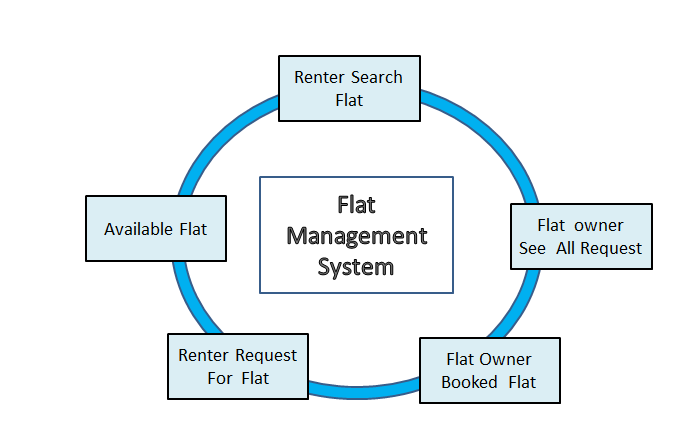
\includegraphics[height=6 cm ,width= 10 cm]{Screenshot (17).png}
\end{frame}
\begin{frame} {Existing System Features}
\begin{itemize}
%\item Login and Logout.
\item Renters search flats/masses manually.
\item Flat owners manually advertising for how many flats are available.
\item Flat owners are manually leafleting their requirements.
\item  Flat owners and renters are manually met for booking flats.
\end{itemize}
\end{frame}
%\item %or you can use a figure to demonstrate the scenario.
%\item mention the problems in the existing process

\begin{frame} {Existing System Problems}

\begin{itemize}
 
    \item Difficulty in finding flats.
    \item Time consuming.
    \item Probability of loosing information.
    \item Maintenance problem.
\end{itemize}
    
\end{frame}

%------------------------------------------------

\section{The Developed System} 

\begin{frame}[t]{Developed System Definition}
%Describe how your developed system problem free, more efficient, user friendly, and cost-effective compared to the existing system.
\textit{"Flat Management System is a web-based application that is designed to booking flats or masses."}
To solve the all existing problems,an online based \textit{Flat Management System} is proposed that works as follows:
\begin{itemize}
\item Users signup online, see all available flats.%you can list some points
\item Flat owners add flats and add their all features in system. %show the workflow of the developed system.
\item Renters search and chose flats.
\item Renters request for booking.%show 1 or 2 WOOOW features of your system.
\item Flat owner chooses renter in site.%in total, slide number must be within six (6).

 

\end{itemize}
\end{frame}
\begin{frame} {Developed System Features}

\begin{itemize}
    \item Flats management.
    \item Booking management.
    \item Renter management.
    \item Time saving.
    \item Efficiency.
    \item Productivity.
\end{itemize}

\end{frame}
\begin{frame}{Developed System Workflow}
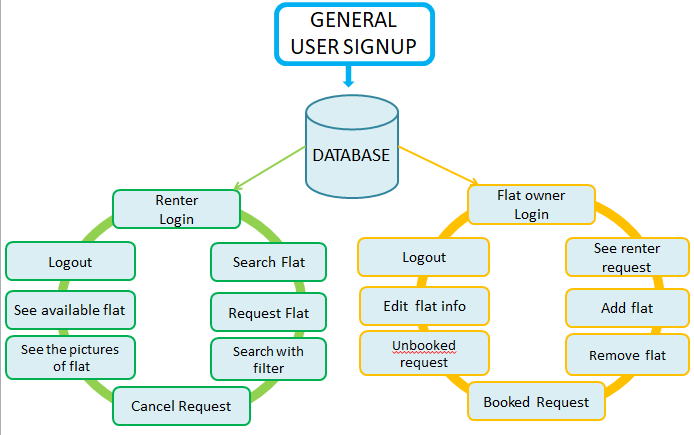
\includegraphics[height=6 cm,width=10 cm]{Screenshot (15).png}
\end{frame}

\begin{frame}{Developed System Workflow}
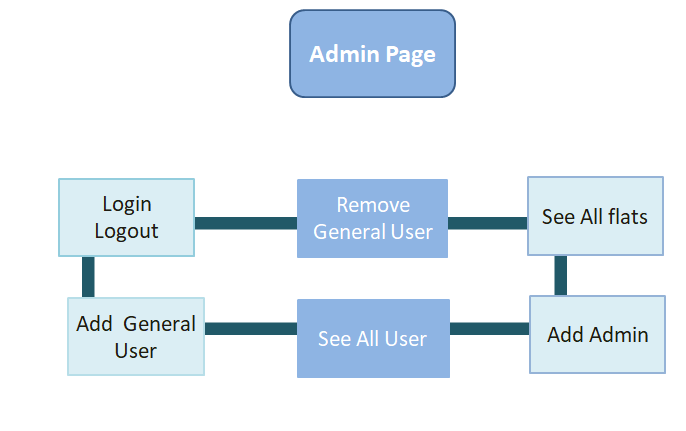
\includegraphics[height=6 cm ,width= 10 cm]{Screenshot (16).png}
\end{frame}

\begin{frame}{WOOW Features}

\begin{itemize}
    \item Collections of all flats.
    \item Search flats by any features.
    \item Request for any flats.
\end{itemize}
    
\end{frame}
%------------------------------------------------

\begin{frame}
\begin{center}
Thank you\\
Contact emails:easyflats@gmail.com
\end{center}
\end{frame}

%------------------------------------------------


%----------------------------------------------------------------------------------------

\end{document} 
